\documentclass[a4paper,12pt]{article}
\usepackage{xltxtra}
\usepackage{fancyhdr}
\usepackage[top=1in, bottom=1.5in, left=1cm, right=1cm]{geometry}
\usepackage{setspace}
\usepackage{bbm}
\usepackage{algorithmicx}
\usepackage{algpseudocode}
\usepackage{algorithm}
\usepackage{graphicx}
\newcommand*\Let[2]{\State #1 $\gets$ #2}
\onehalfspacing
% Chestiile pentru mate
\usepackage{amsmath}
\usepackage{amsfonts}
\usepackage{bbm}
\author{Roland Szabo, gr. 235}
\usepackage{fancyhdr}
\pagestyle{fancy}
\makeatletter
\makeatother
\lhead{Roland Szabo, gr. 235}
\rhead{Lab 4, 4.12.13}
\begin{document}

\section{Problem statement}
Implement the classical algorithm for factoring integers and Pollard's p - 1 algorithm.

Do a running time analysis of the two algorithms. 

\section{Algorithms}
	
\subsection{Trial division}
	\begin{algorithmic}
		\Procedure{trial}{a}
			\For{$ i = 2, \sqrt{n} $}
				\If {$ a \mod i = 0$}
					\Let{trial}{i}
				\EndIf
			\EndFor
		\EndProcedure	
	\end{algorithmic}
	
\subsection{Pollard's p - 1}
	\begin{algorithmic}
		\Procedure{pollard}{n, b}
			\Let{k}{$lcm(1, ..., b)$}
			\Let{a}{$random(1,n-1)$}
			\Let{a}{$ a^k \mod n $}
			\Let{d}{$gcd(a-1,n)$}
			\If{d=1 or d = n}
				\Let{trial}{n}
			\Else
				\Let{trial}{d}
			\EndIf
		\EndProcedure	
	\end{algorithmic}
	
	
\section{Runtime analysis}

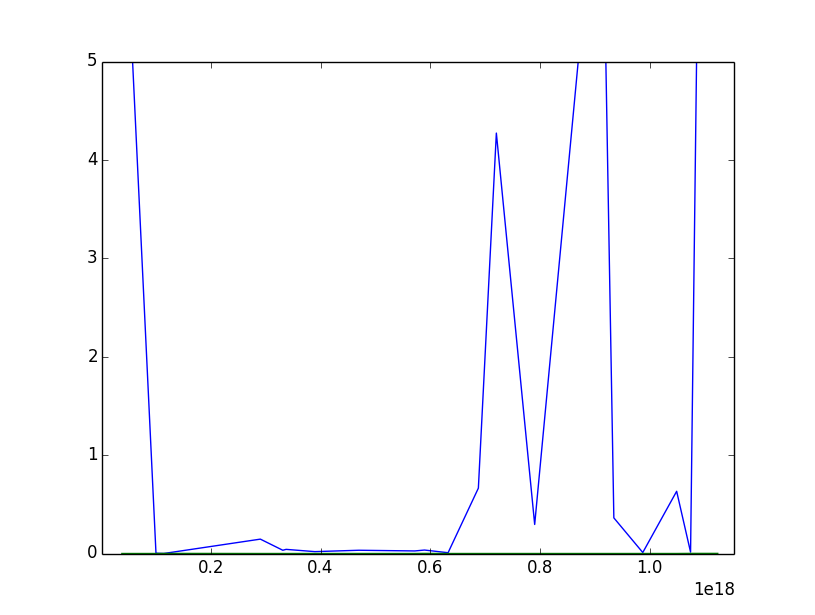
\includegraphics{figure_1.png}

As can be seen from the graph, the naive, brute-force algorithm has an exponential complexity when the numbers are primes, or have only large divisors. Pollard's p-1 method is very fast, but it doesn't find all factors.

\end{document}